\section{Results}

\subsection{Variation in observed hospital thrombolysis use}

Thrombolysis use in the original data varied between hospitals from 1.5\% to 24.3\% of all patients, and 7.3\% to 49.7\% of patients arriving within 4 hours of known (precise or estimated) stroke onset.

%%%%%%%%%%%%%%%%%%%%%%%%%%%%%%%%%%%%%%%%%%%%%%%%%%%%%%%%%%%%%%%%%%%%%%%%

\subsection{Feature selection}

A model using  10 features had an ROC AUC of 0.923, compared to 0.922 for a model using all available features. We selected 10 features for all subsequent work, which were (in order of selection):

\begin{itemize}
    \item \emph{Arrival-to-scan time} (minutes)
    \item \emph{Infarction}: Stroke type (1 = infarction, 0 = haemorrhage)
    \item \emph{Stroke severity} (NIHSS on arrival)
    \item \emph{Precise onset time} (1 = precise, 0 = best estimate)
    \item \emph{Prior disability level} (mRS before stroke)
    \item \emph{Stroke team}
    \item \emph{Use of anticoagulants} (prior to stroke onset; 1 = Yes, 0 = No)
    \item \emph{Onset-to-arrival time} (minutes)
    \item \emph{Onset during sleep }(1 = Yes, 0 = No)
    \item \emph{Age} (midpoint of 5 year age bands)
\end{itemize}

Correlations between the 10 features were measured. All r-squared were less than 0.05 except a) age and prior disability level (r-squared 0.146), and b) onset during sleep and precise onset time (r-squared 0.078).

%%%%%%%%%%%%%%%%%%%%%%%%%%%%%%%%%%%%%%%%%%%%%%%%%%%%%%%%%%%%%%%%%%%%%%%%

\subsubsection{Model accuracy}

Model accuracy was measured using stratified 5-fold cross validation. Overall accuracy was 85.0\% (83.9\% sensitivity and specificity could be achieved simultaneously). The model predicted hospital thrombolysis use at each hospital with very good accuracy (r-squared = 0.977, with a mean absolute error of 1.1 percentage points). The appendix contains further model accuracy analysis.

%%%%%%%%%%%%%%%%%%%%%%%%%%%%%%%%%%%%%%%%%%%%%%%%%%%%%%%%%%%%%%%%%%%%%%%%
\subsection{Individual patient SHAP values}
SHAP values are calculated as how they affect log odds of receiving thrombolysis, but for individual predictions, probability values are more intuitive. Figure \ref{fig:results_waterfall} shows \emph{waterfall} plots for example patients with low and high probability of receiving thrombolysis. Waterfall plots show the influence of features for an individual prediction (in our case, patient). The SHAP model starts with a base prediction of a 24\% probability of receiving thrombolysis, before feature values are taken into account. For the patient with a low probability of receiving thrombolysis, the two most influential features reducing the probability of thrombolysis were a long arrival-to-scan time (138 minutes) and a low stroke severity (NIHSS=2). For the patient with a high probability of receiving thrombolysis, the two most influential features increasing the probability of thrombolysis were a short arrival-to-scan time (17 minutes) and a moderate stroke severity (NIHSS=14). 

\begin{figure}%[!ht]
    \caption*{\footnotesize{\textsf{Patient with low probability of receiving thrombolysis}}}
    \vspace{-4mm} % reduce space after caption
    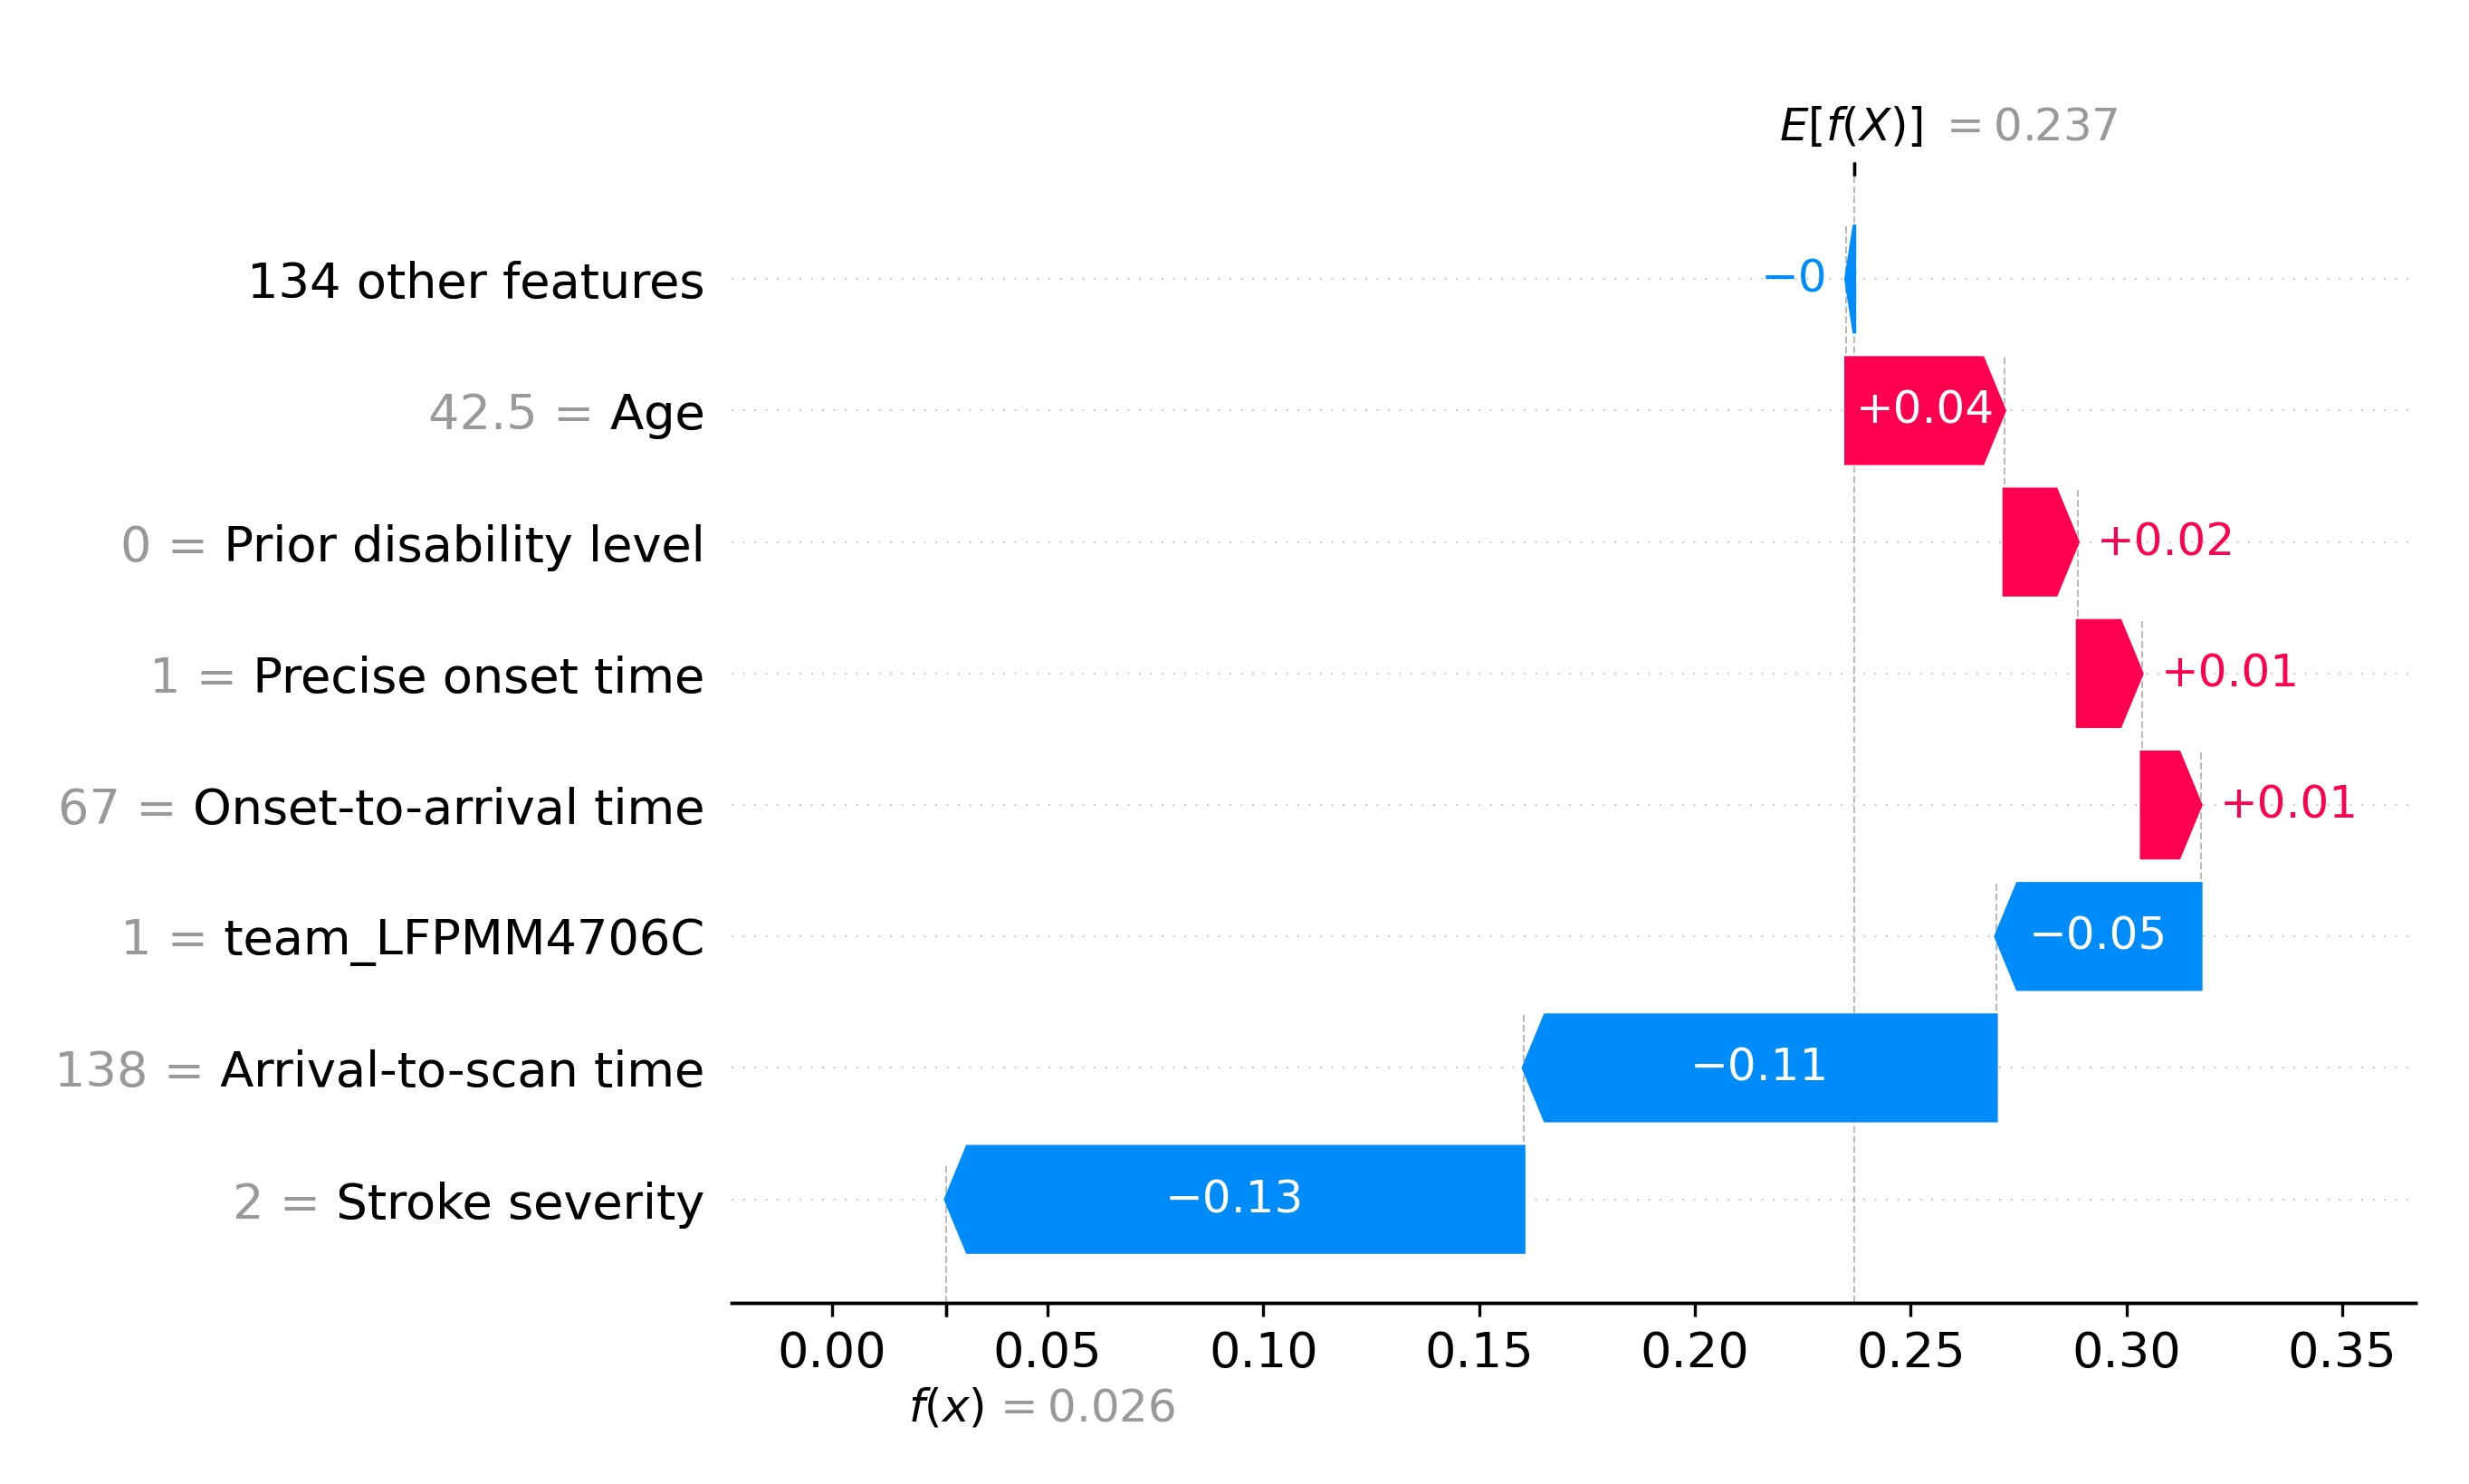
\includegraphics[width=0.75\textwidth]{./images/03_xgb_10_features_waterfall_probability_low}
    \vspace{2mm}
    \caption*{\footnotesize{\textsf{Patient with high probability of receiving thrombolysis}}}
    \vspace{-4mm} % reduce space after caption
    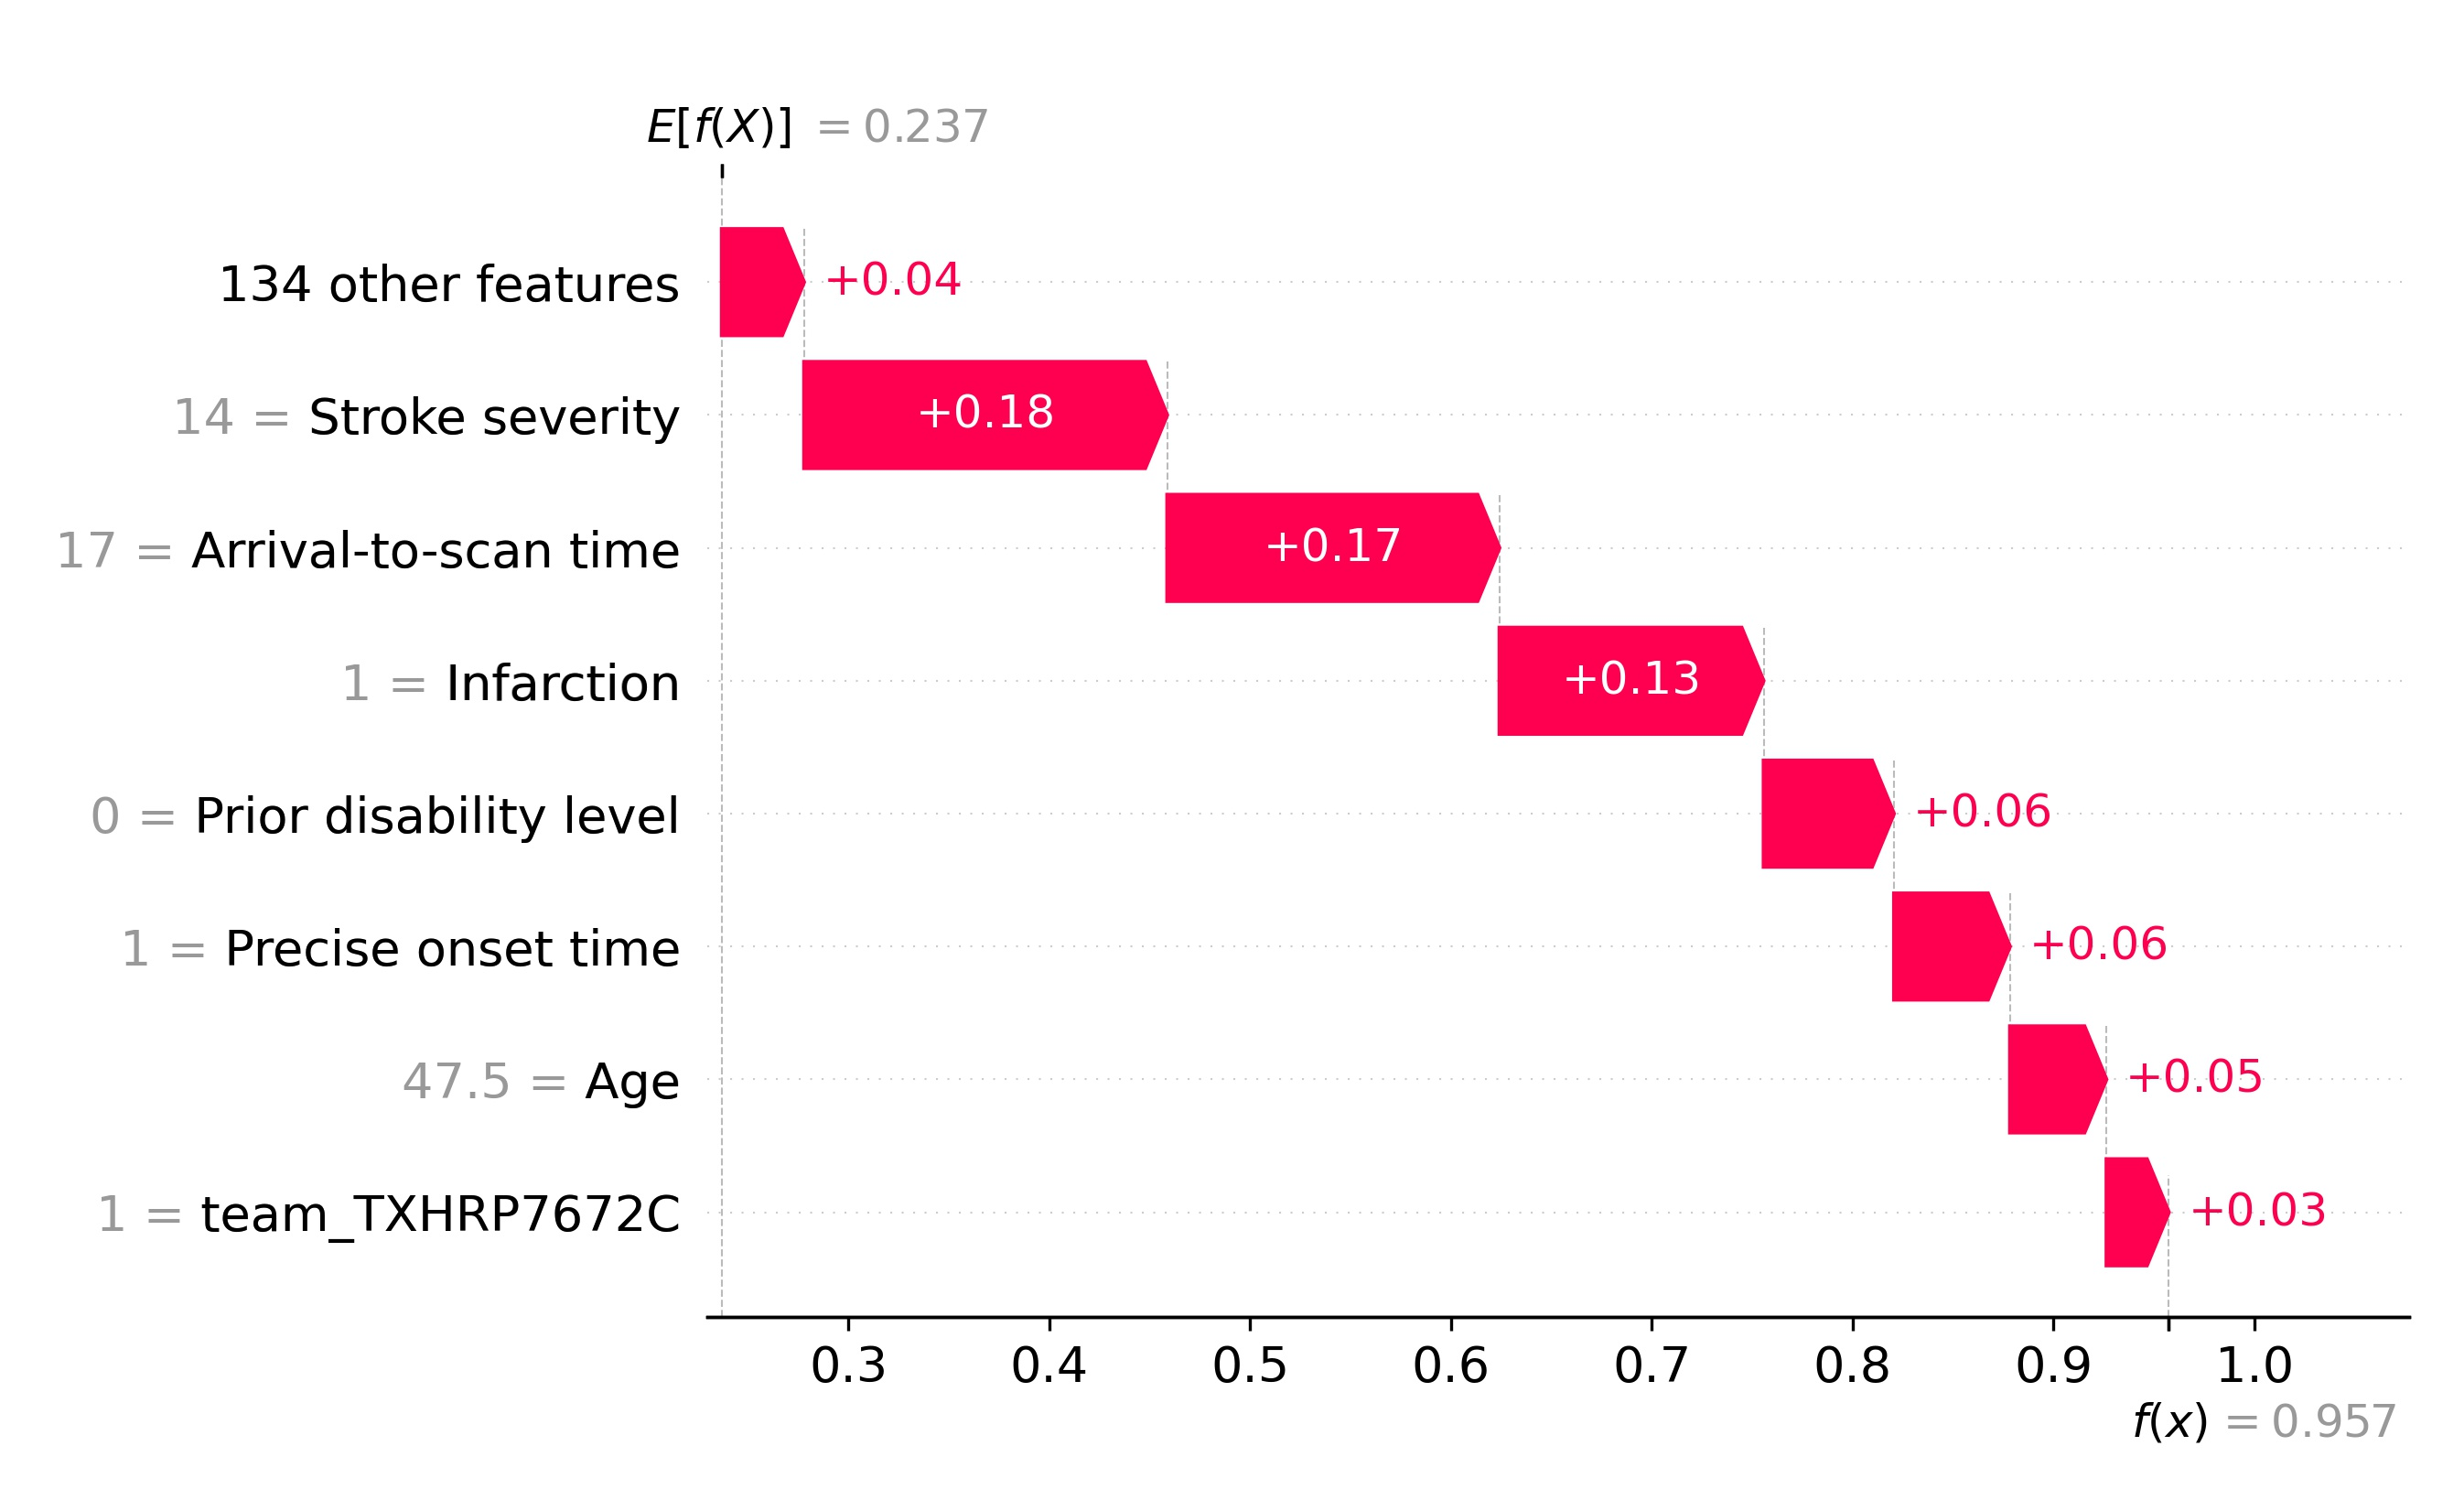
\includegraphics[width=0.75\textwidth]{./images/03_xgb_10_features_waterfall_probability_high}
\caption{Waterfall plots showing the influence of each feature on the predicted probability of a single patient receiving thrombolysis. Top: An example of a patient with a low probability (2.6\%) of receiving thrombolysis. Bottom: An example of a patient with a high probability (95.7\%) of receiving thrombolysis.}
\label{fig:results_waterfall}
\end{figure}

%\newpage
%%%%%%%%%%%%%%%%%%%%%%%%%%%%%%%%%%%%%%%%%%%%%%%%%%%%%%%%%%%%%%%%%%%%%%%%

\subsection{The relationship between feature values and the odds of receiving thrombolysis}

\begin{minipage}{1\textwidth}
Figure \ref{fig:shap_feature_subfigure} shows the relationship between patient level feature values and their SHAP values. Key observations are:

\begin{itemize}
    \item \emph{Stroke type}: The SHAP values for stroke type show that the model effectively eliminated any probability of receiving thrombolysis for haemorrhagic stroke.
    \item \emph{Arrival-to-scan time}: The odds of receiving thrombolysis reduced by 9-fold over the first 120 minutes of arrival-to-scan time.
    \item \emph{Stroke severity (NIHSS)}: The odds of receiving thrombolysis were lowest at NIHSS 0, increased and peaked at NIHSS 15-25, and then fell again with higher stroke severity (NIHSS above 25). The difference between minimum odds and maximum odds of receiving thrombolysis was 30-fold.
    \item \emph{Stroke onset time type}: The odds of receiving thrombolysis were 3-fold greater for precise onset time than estimated onset time.
    \item \emph{Disability level (mRS) before stroke}: The odds of receiving thrombolysis fell 6-fold between mRS 0-5.
    \item \emph{Use of AF anticoagulants}: The odds of receiving thrombolysis were reduced 5-fold with anticoagulant use.
    \item \emph{Onset-to-arrival time}: The odds of receiving thrombolysis were similar below 120 minutes, then fell 3-fold between 120-240 minutes.
    \item \emph{Age}: The odds of receiving thrombolysis were similar below 80 years old, then fell 2-fold between 80-110 years old.    
    \item \emph{Onset during sleep}: The odds of receiving thrombolysis were 4-fold lower for onset during sleep.
    \item \emph{Hospital attended}: There was a 13-fold difference in odds of receiving thrombolysis between hospitals.
\end{itemize}
\end{minipage}

% SHAP violon plots

\begin{figure}%[!h]
\centering
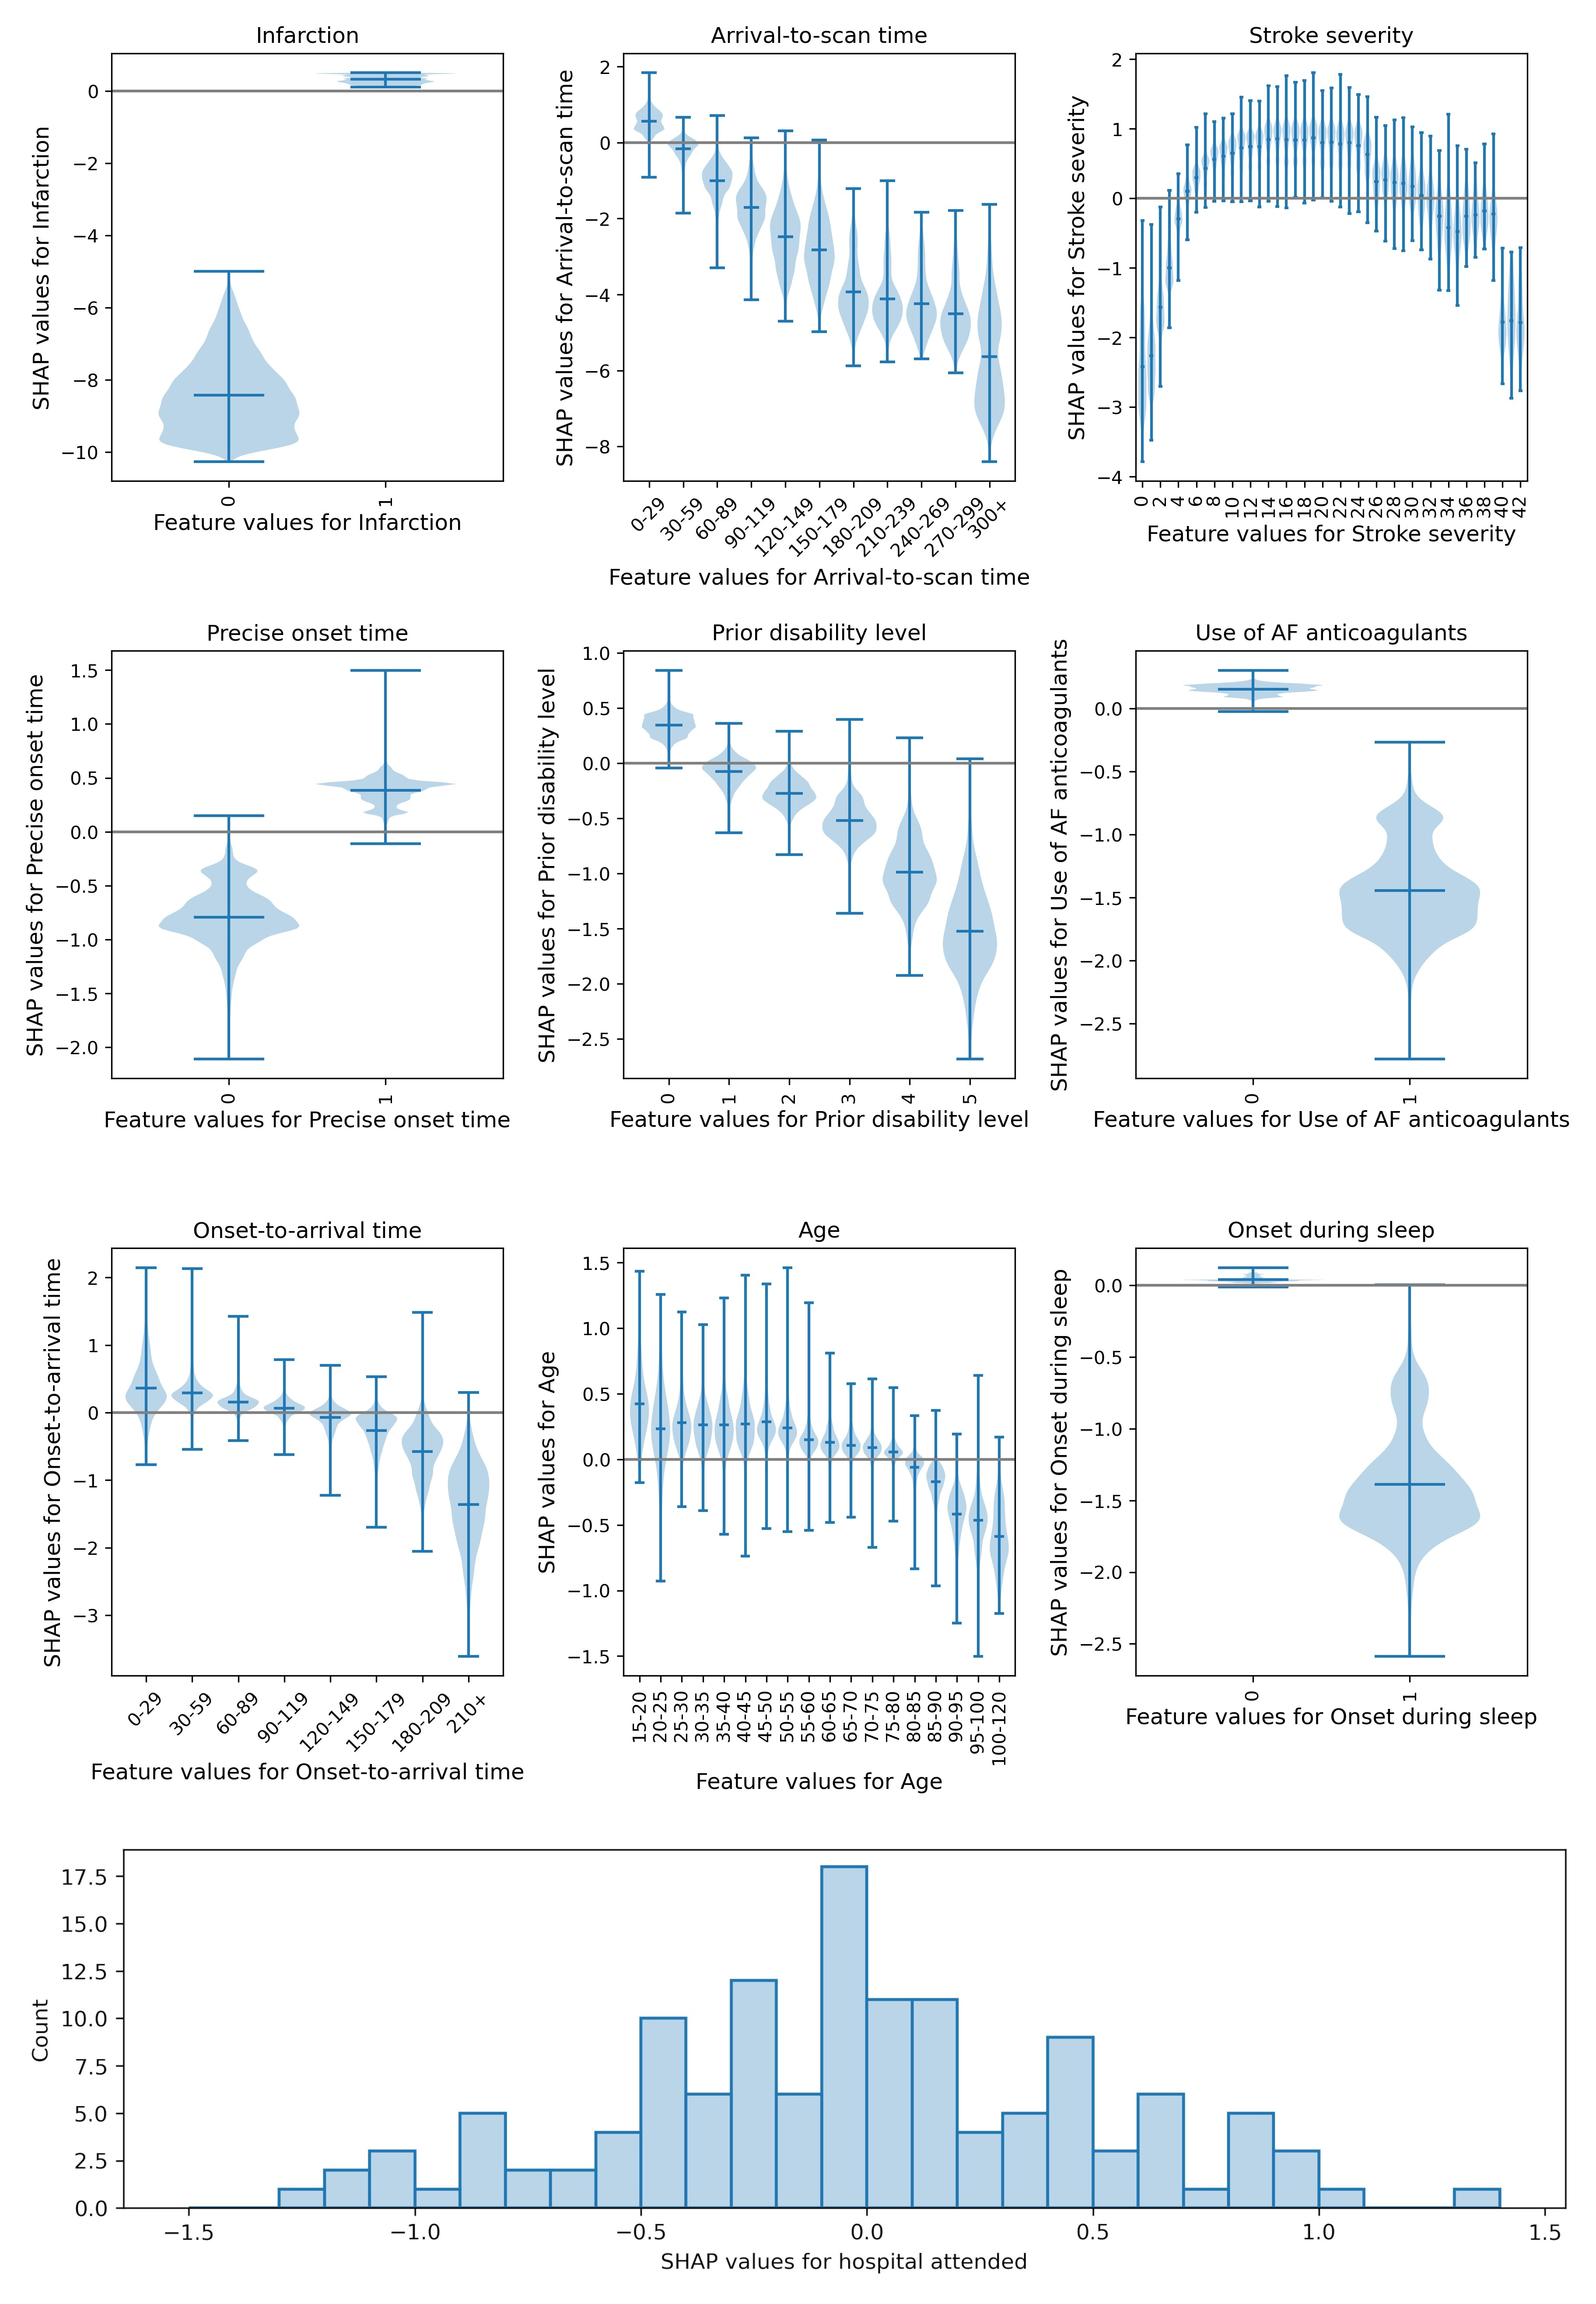
\includegraphics[width=0.9\textwidth]{./images/03a_combined_shap}
\caption{Plots showing the relationship between SHAP values and feature values. Top: Violin plots showing the relationship between SHAP values and feature values. The horizontal line shows the median SHAP value. The plots are ordered in ranked feature importance (using the mean absolute SHAP value across all instances). Bottom: Histogram showing the frequency of SHAP values for the hospital attended.}
\label{fig:shap_feature_subfigure}
\end{figure}

%%%%%%%%%%%%%%%%%%%%%%%%%%%%%%%%%%%%%%%%%%%%%%%%%%%%%%%%%%%%%%%%%%%%%%%%

\subsection{Investigating how the identity of a hospital influences thrombolysis rate}

The mean hospital SHAP main effect value correlated with the observed hospital thrombolysis rate with an r-squared of 0.558 (figure \ref{fig:shap_correlation}, left), suggesting that 56\% (P$<$0.0001) of the between-hospital variance in thrombolysis use may be explained by the attended hospitals' SHAP main effect values, i.e. the hospitals' predisposition and/or preparedness to use thrombolysis.

Using the \emph{10k holdout} model, the predicted use of thrombolysis across the 132 hospitals for the identical 10k cohort of patients ranged from 10\% to 45\%. The mean hospital SHAP main effect value for the 10k cohort correlated very closely with the predicted thrombolysis use in the 10k cohort at each hospital (r-squared of 0.971, figure \ref{fig:shap_correlation}, right), confirming that the hospital SHAP main effect value is providing direct insight into hospitals' propensity to use thrombolysis.

\begin{figure}[!h]
\centering
\begin{subfigure}{.49\textwidth}
  \centering
    \caption*{\footnotesize{\textsf{Observed thrombolysis}}}
    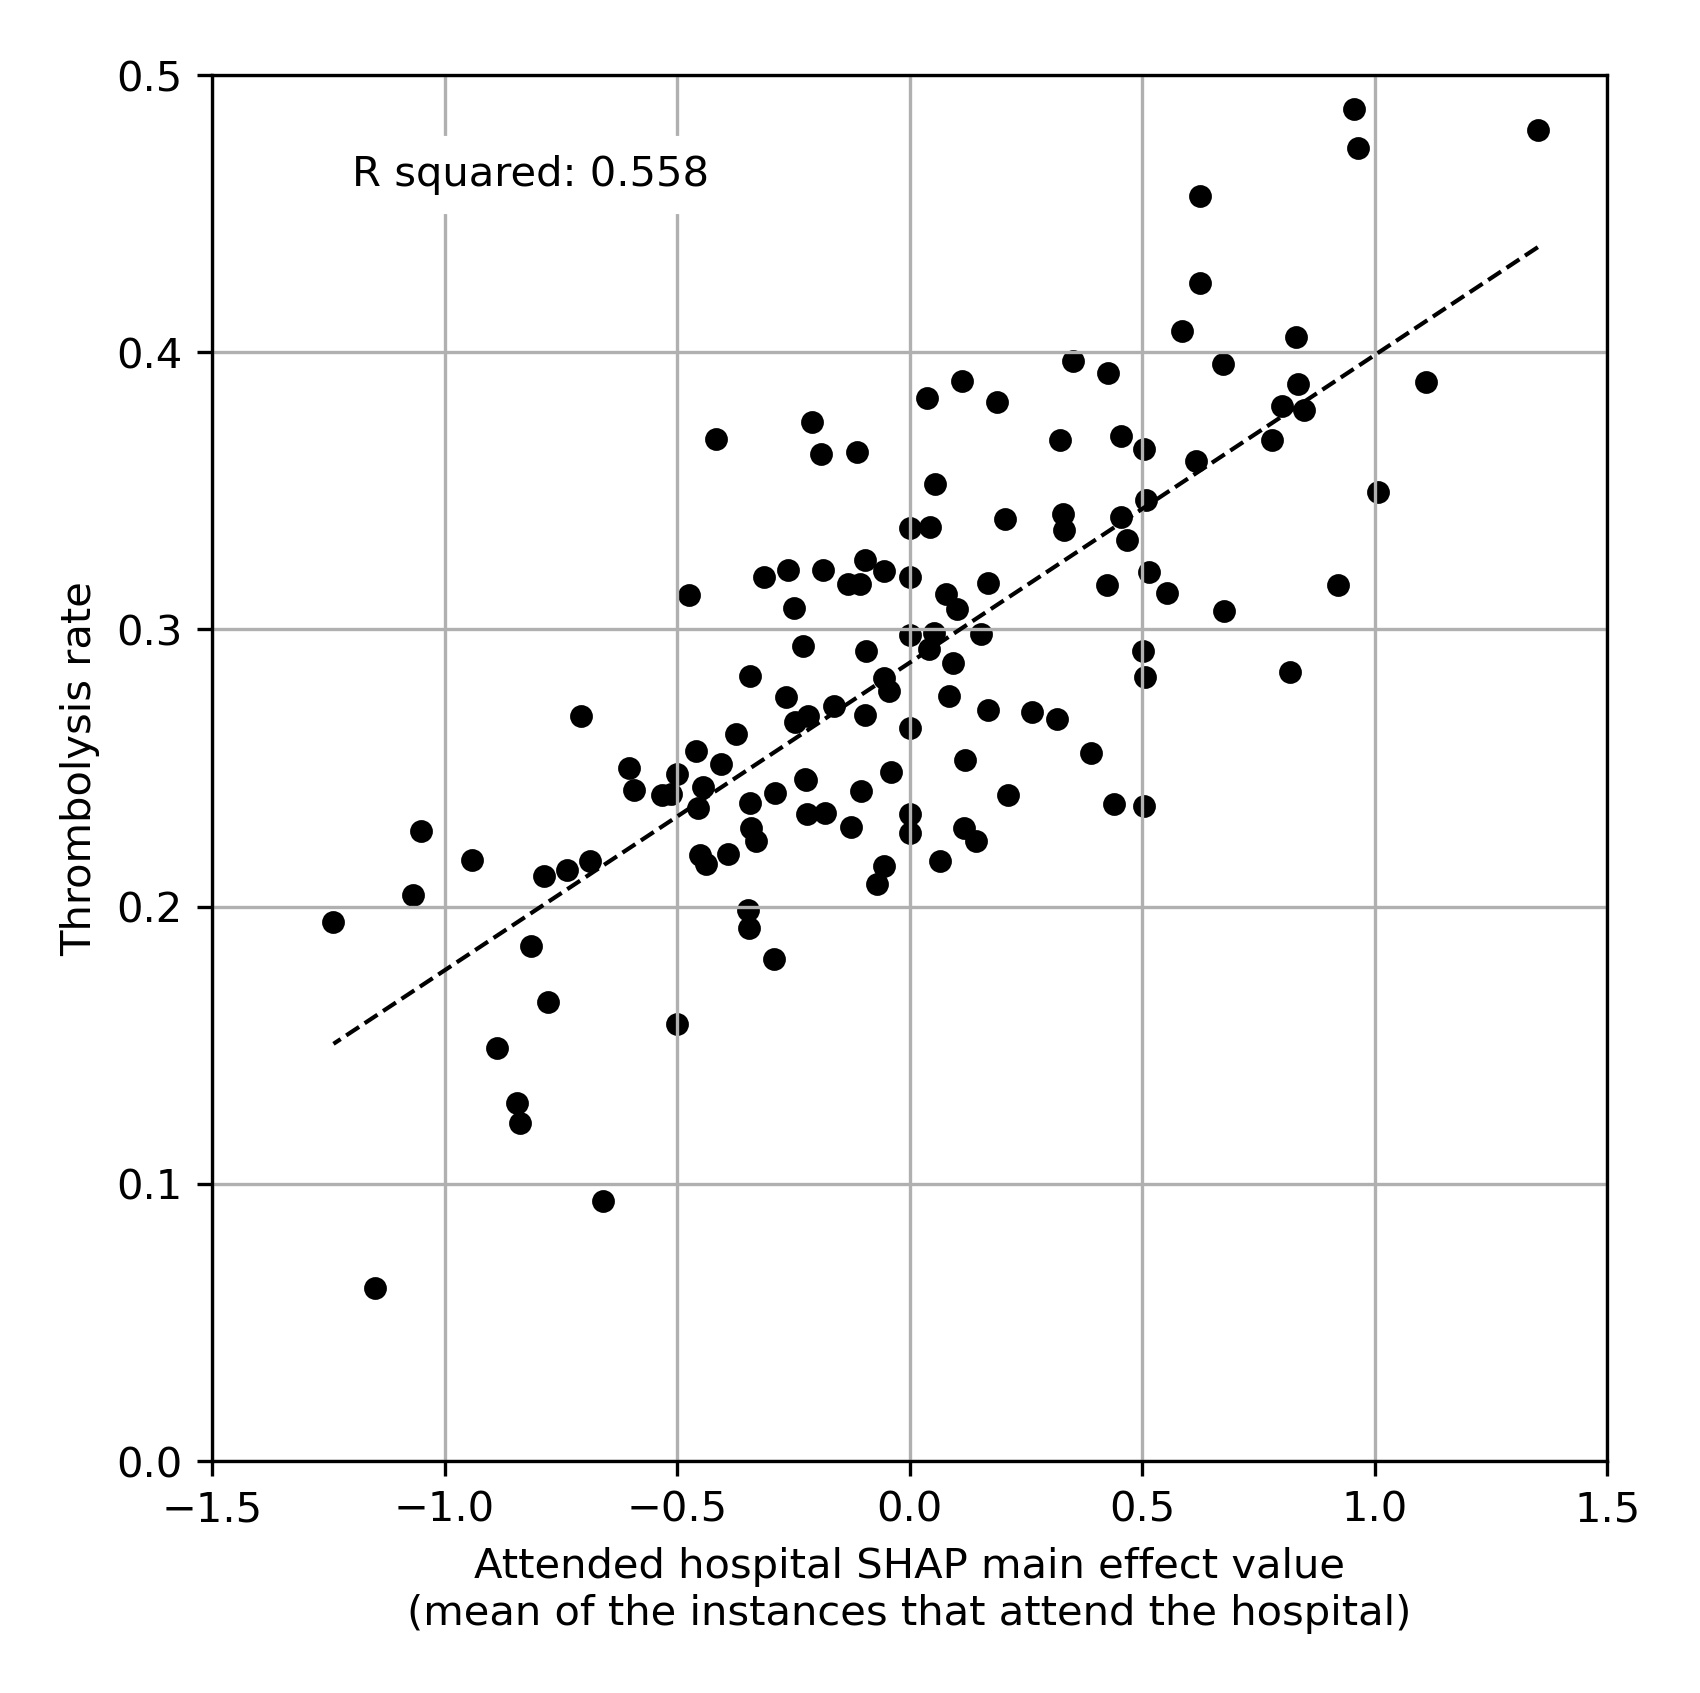
\includegraphics[width=0.9\textwidth]{./images/03c_xgb_10_features_attended_hosp_shap_maineffect_vs_ivt_rate}
\end{subfigure}
\begin{subfigure}{.49\textwidth}
  \centering
    \caption*{\footnotesize{\textsf{Predicted 10K thrombolysis}}}
    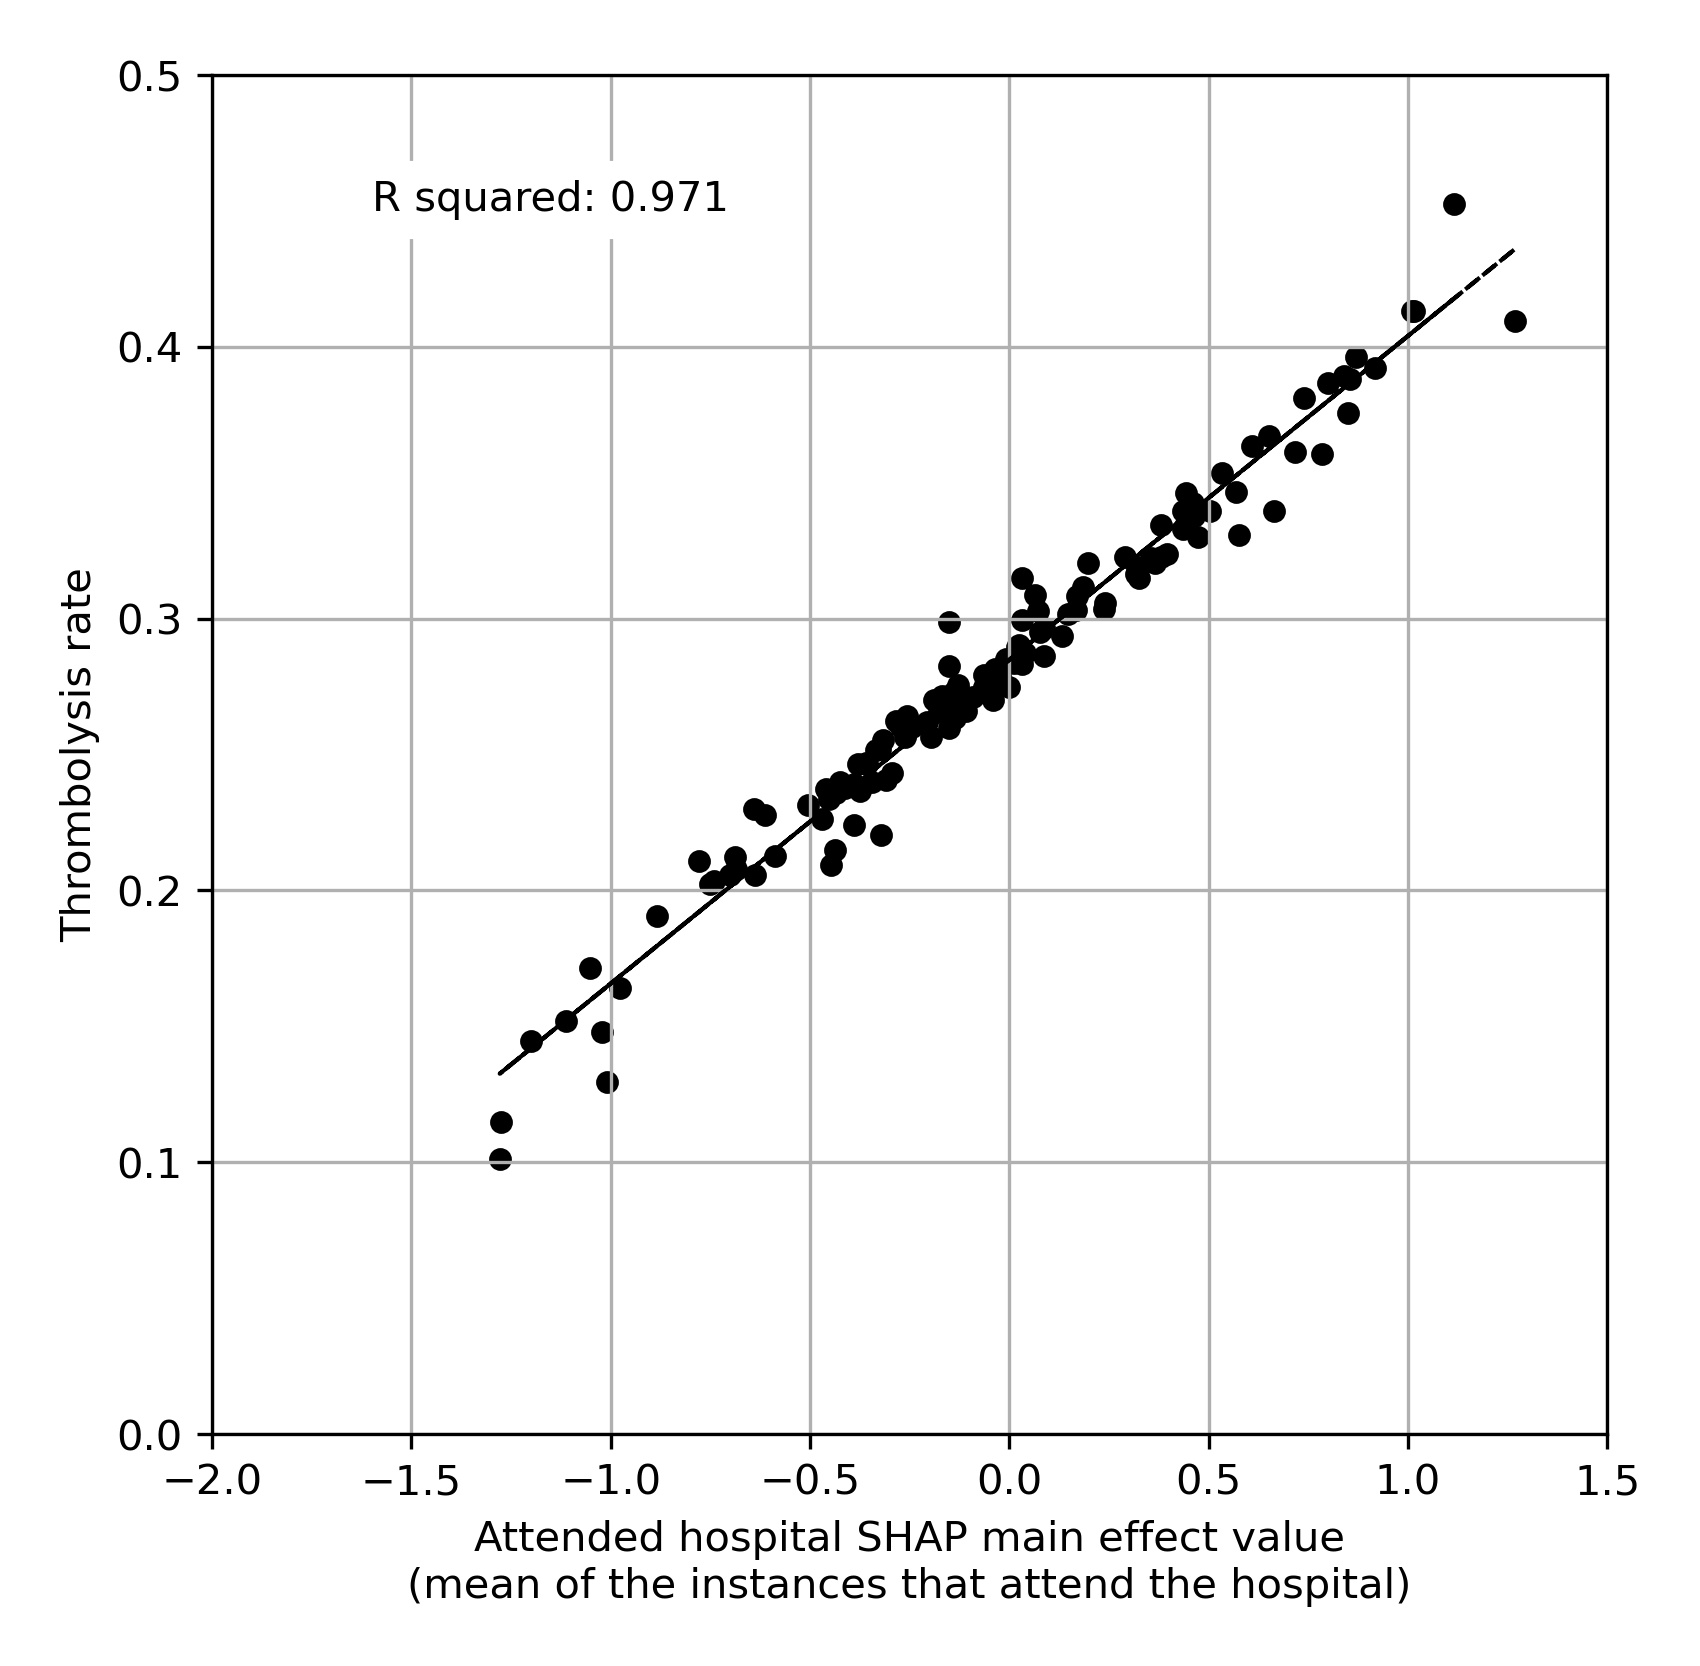
\includegraphics[width=0.9\textwidth]{./images/04a_xgb_10_features_10k_cohort_attended_hosp_shap_maineffect_vs_ivt_rate}
\end{subfigure}

\caption{Correlations between hospital SHAP main effect value and the observed thrombolysis use at each hospital. Left: Observed thrombolysis (using the \emph{all data} model). Right: Predicted 10k cohort thrombolysis rate (using the \emph{10k holdout} model)}
\label{fig:shap_correlation}
\end{figure}
%%%%%%%%%%%%%%%%%%%%%%%%%%%%%%%%%%%%%%%%%%%%%%%%%%%%%%%%%%%%%%%%%%%


%\newpage
\subsection{Investigating how patient populations and hospital identity and processes influences thrombolysis rate}

We predicted thrombolysis use using mean subset SHAP values for patients attending each hospital. Figure \ref{fig:shap_multiple_regression} shows that 36\% (P$<$0.0001) of the variance in observed between-hospital thrombolysis use can be explained by the patient population, 74\% (P$<$0.0001) can be explained by hospital identity and processes, and that 95\% (P$<$0.0001) can be explained by the combined information from both the patient population and hospital identity and processes. 

\begin{figure}[!h]
    \centering
    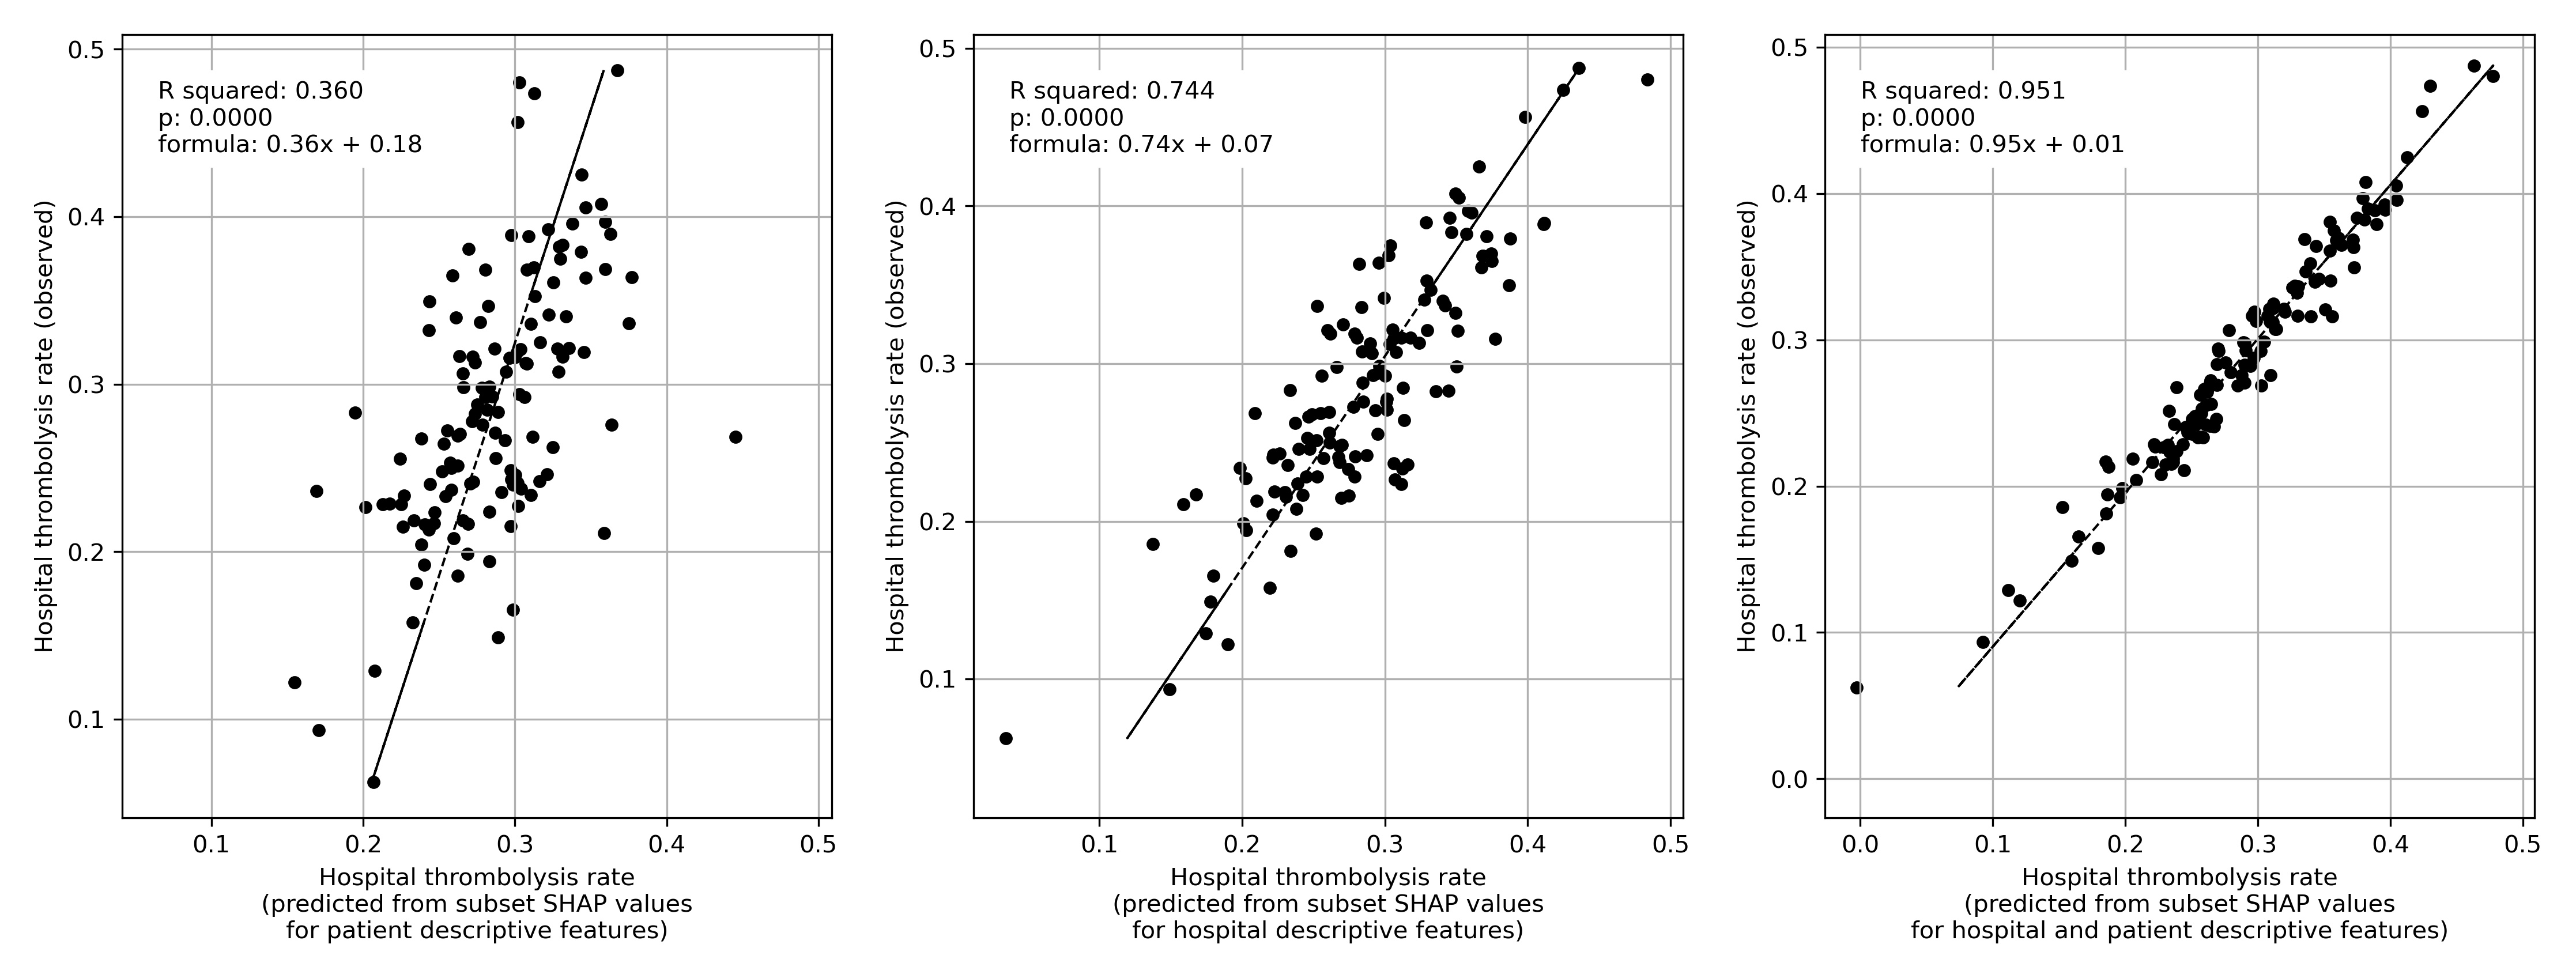
\includegraphics[width=0.9\textwidth]{./images/03f_xgb_10_features_multiple_regression_patient_hospital}
    \caption{Multiple regression of subset SHAP values (mean of patients attending hospital) with hospital observed thrombolysis rate (using the \emph{all data} model). Left: Subset SHAP values for the eight patient descriptive features (age, stroke severity, prior disability, onset-to-arrival time, stroke type, type of onset time, anticoagulants, and onset during sleep). Middle: Subset SHAP values for the two hospital descriptive features (arrival-to-scan time, and hospital attended). Right: Subset SHAP values for all 10 features (for both hospital and patient descriptive features).}
  \label{fig:shap_multiple_regression}
\end{figure}

%%%%%%%%%%%%%%%%%%%%%%%%%%%%%%%%%%%%%%%%%%%%%%%%%%%%%%%%%%%%%%%%%%%%%%%%
%\newpage
\subsection{Variation in hospital thrombolysis use for patient subgroups}

Figure \ref{fig:results_boxplot} shows observed and predicted use of thrombolysis, broken down by patient subgroup. The subgroups of patients with one defined non-ideal feature all had reduced thrombolysis use than the complete patient population, and combining these non-ideal features reduced thrombolysis use further. There was, however, significant variation between hospitals' thrombolysis use in each of these subgroups. The observed and predicted thrombolysis use show the same general patterns.

\begin{figure}[!h]
\centering
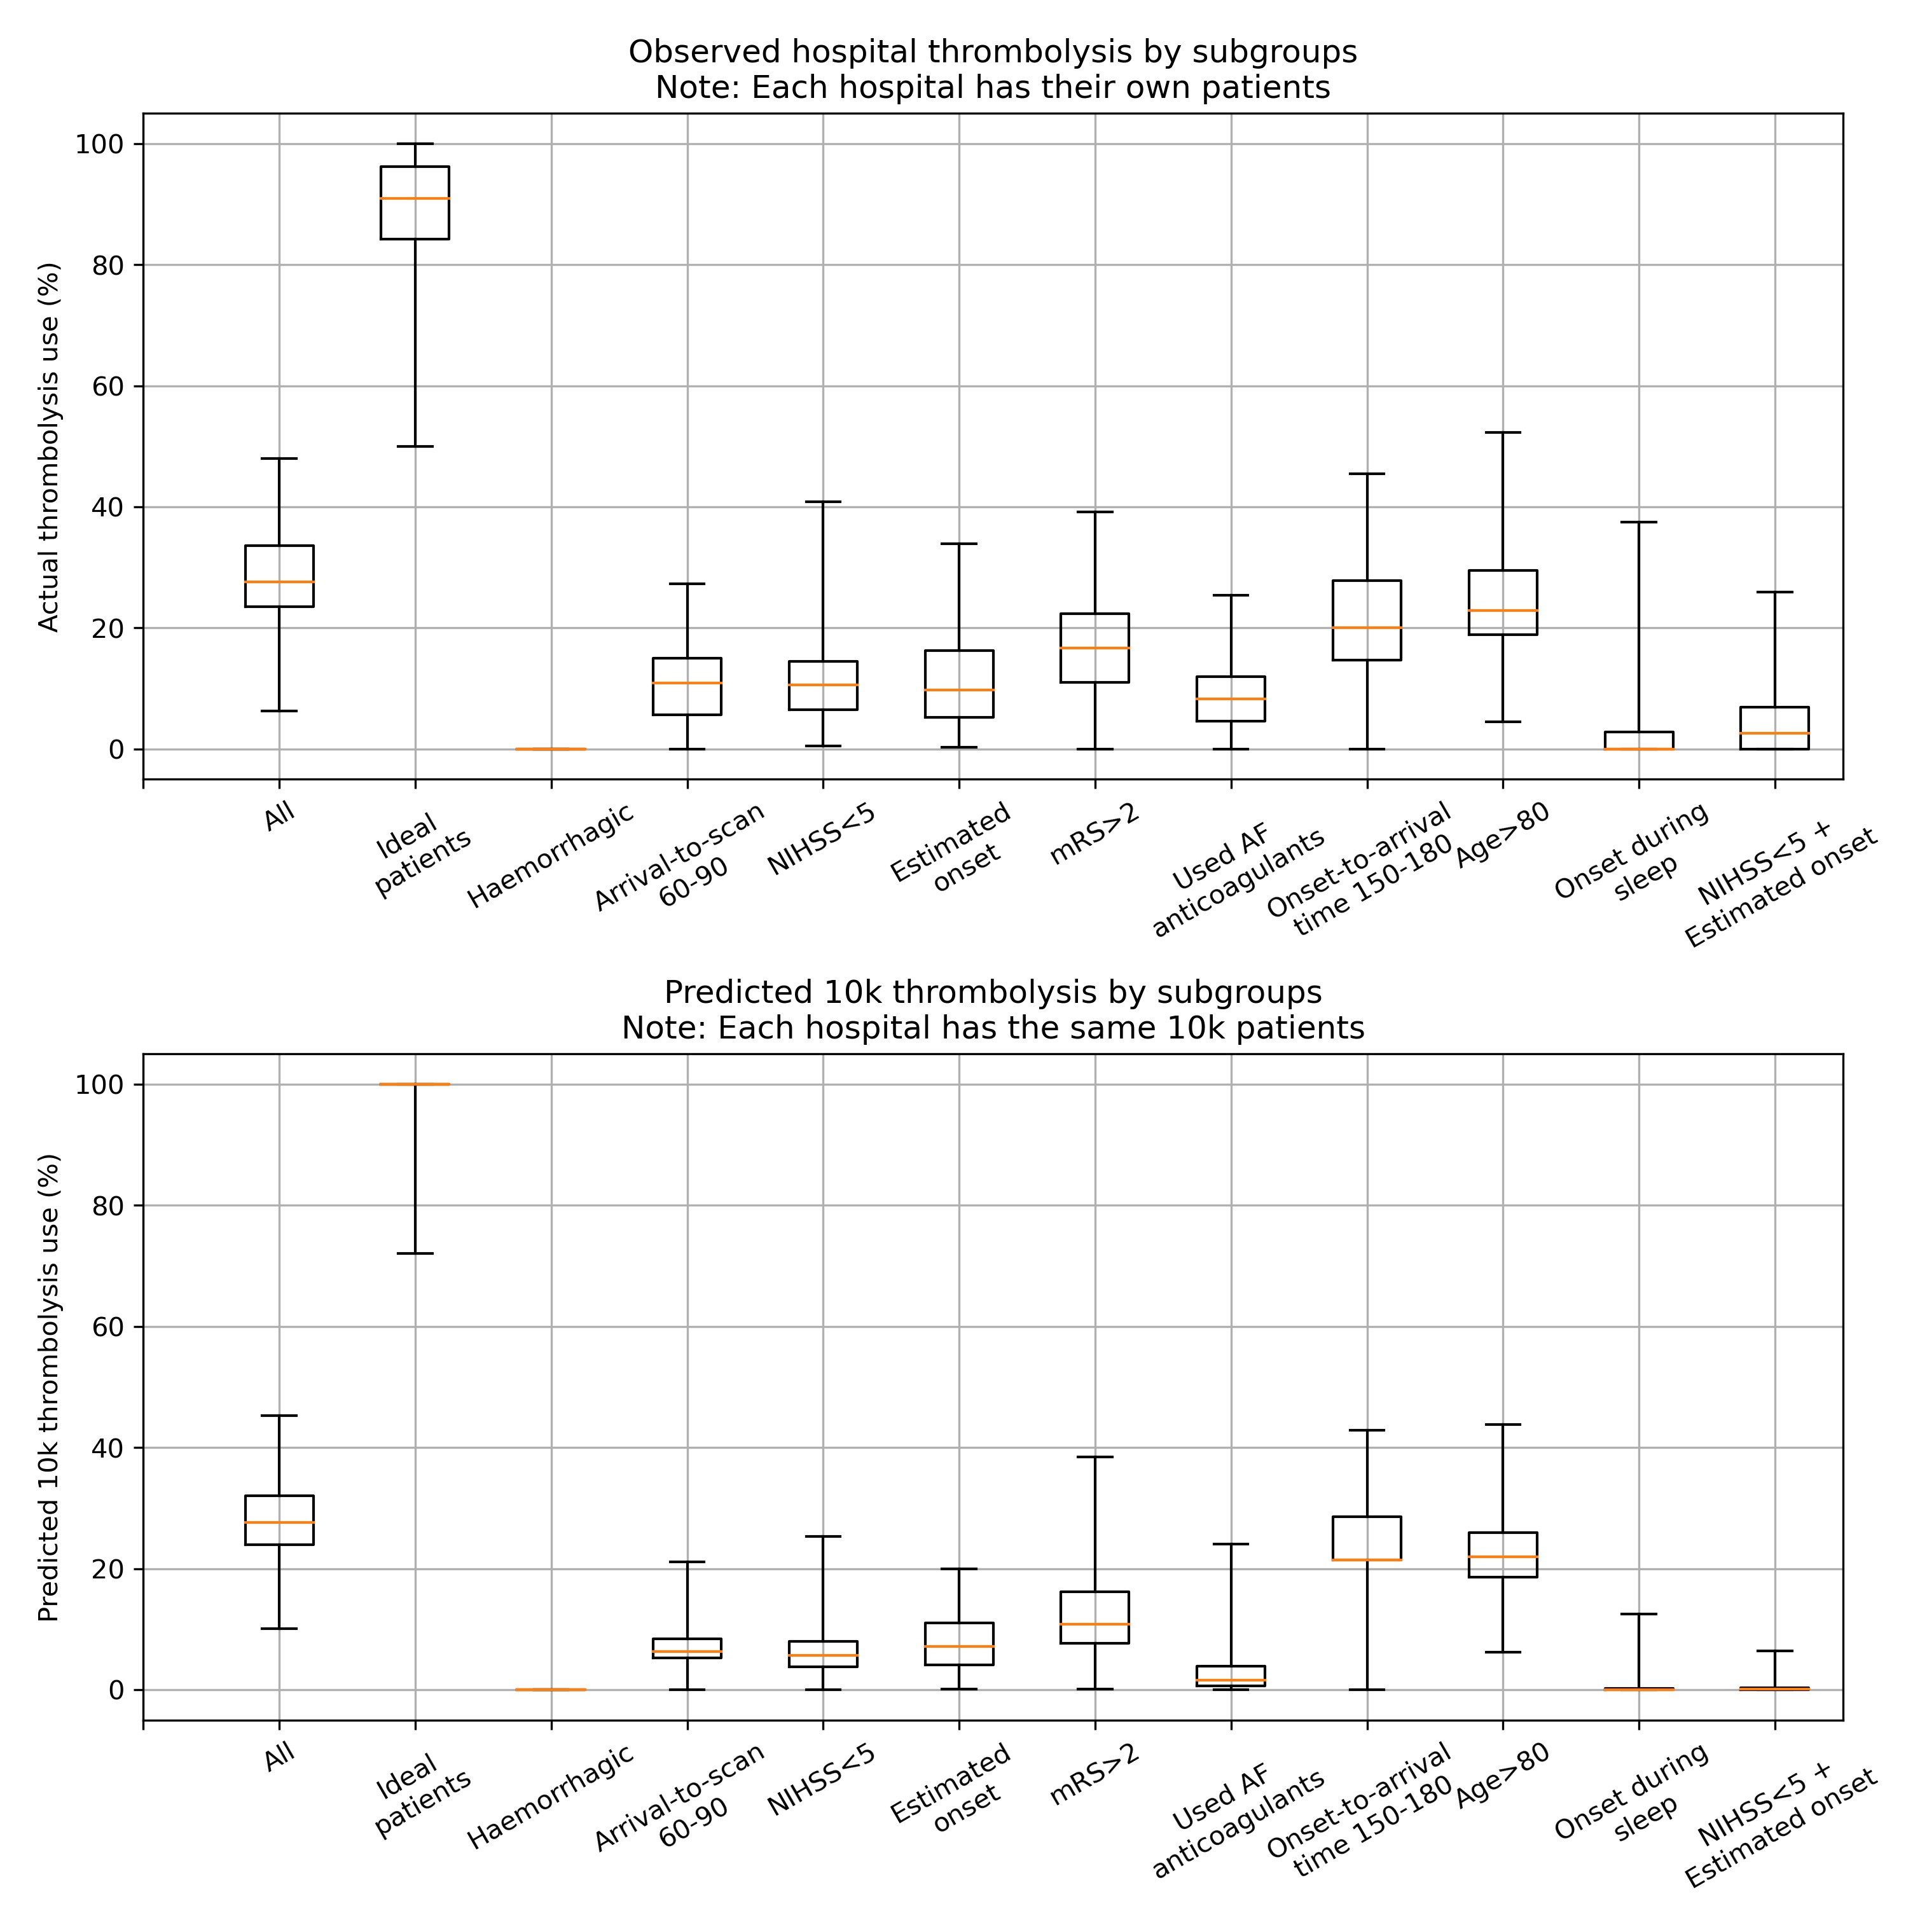
\includegraphics[width=0.75\textwidth]{./images/04c_xgb_10_features_10k_cohort_actual_vs_modelled_subgroup_boxplot}
\caption{Boxplot for either observed (top) or predicted (bottom) use of thrombolysis for subgroups of patients. The `ideal patients' subgroup has a mid-level stroke severity (NIHSS 10-25), short arrival-to-scan time ($<$30 minutes), stroke caused by infarction, precise stroke onset time known, no pre-stroke disability (mRS 0), not taking any atrial fibrillation anticoagulants, short onset-to-arrival time ($<$90 minutes), $<$80 years old, and onset not during sleep. The single features are ordered in ranked feature importance (using the mean absolute SHAP value across all instances).}
\label{fig:results_boxplot}
\end{figure}